% Provenance (never printed): see sources/outline_sources.md (Year 1: optical
% mineralogy with the polarising microscope; Michel-Levy chart). Interference
% colours in figdata/bachelor-1/michel_levy.py from the CIE 1931 colour-matching
% functions and illuminant D65 (data/derived/bachelor-1-cie*.csv); exercise and
% problem values in the Book 3 scratch calculator calc/ch08.py.
\chapter{Mineralogi optik}\label{ch:b1:optical-mineralogy}

Di antara polarisator silang, \omterm{def:b1:field-lab-methods-1:thin-section}{sayatan tipis} gabro menyala seperti kaca patri. Balok-balok panjang abu-abu dan putih, bergaris seperti kode batang, melintasi medan; di antaranya, butir-butir berpendar biru, kuning, dan magenta; beberapa tetap hitam apa pun sudutnya. Setiap efek ini memiliki penyebab yang dapat dihitung, dan masing-masing menunjukkan \omterm{def:b1:rock-forming-minerals:mineral}{mineral} apa yang ada di sana. Bab ini menjelaskan bagaimana cahaya melintasi kristal, mengapa \omterm{def:b1:rock-forming-minerals:mineral}{mineral} di antara polarisator silang berwarna, bagaimana warna itu mengukur sifat \omterm{def:b1:rock-forming-minerals:mineral}{mineral}, dan bagaimana seorang petrolog menamai butir-butir \omterm{def:b1:field-lab-methods-1:thin-section}{sayatan tipis} hanya dengan mikroskop. Bab ini diakhiri dengan sayatan tak dikenal, yang \omterm{def:b1:rock-forming-minerals:mineral}{mineral-mineralnya} dan \omterm{def:b1:cross-sections:thickness}{ketebalan sebenarnya} ditemukan dari apa yang ditampilkannya.

\begin{recall}
\omterm{def:b1:field-lab-methods-1:thin-section}{Sayatan tipis} adalah irisan batuan setebal sekitar \qty{30}{\micro m} pada kaca objek; \omterm{def:b1:field-lab-methods-1:microscope}{mikroskop polarisasi} melihatnya dalam \omterm{def:b1:field-lab-methods-1:microscope}{cahaya terpolarisasi bidang} (satu polarisator) dan di antara polarisator silang (\cref{ch:b1:field-lab-methods-1}). Indeks bias $n$ suatu medium adalah perbandingan laju cahaya dalam vakum terhadap lajunya dalam medium, dan pembiasan pada suatu antarmuka mematuhi hukum Snell $n_1\sin i_1 = n_2\sin i_2$ (fisika, Sarjana Tahun ke-1). Cahaya adalah gelombang transversal; sebuah polarisator hanya meneruskan komponen medan listrik sepanjang arahnya, sehingga analisator pada sudut $\alpha$ terhadapnya meneruskan pecahan $\cos^2\alpha$ dari intensitas (hukum Malus, fisika).
\end{recall}

\section{Cahaya dalam kristal}

Dalam kaca, cairan, atau kristal kubik, cahaya merambat dengan laju yang sama di setiap arah dan apa pun arah getarnya. Pada sebagian besar \omterm{def:b1:rock-forming-minerals:mineral}{mineral} tidak demikian: susunan atom berbeda sepanjang arah yang berbeda, dan begitu pula tanggapan elektron terhadap medan listrik gelombang.

\begin{definition}[Mineral isotropik dan anisotropik]\label{def:b1:optical-mineralogy:anisotropic}
Sebuah \omterm{def:b1:rock-forming-minerals:mineral}{mineral} adalah \emph{mineral isotropik}\index{mineral isotropik} bila indeks biasnya sama untuk setiap arah rambat dan getaran cahaya; \omterm{def:b1:rock-forming-minerals:mineral}{mineral} kubik (\omterm{def:b1:rock-forming-minerals:groups}{garnet}, halit, spinel) dan kaca bersifat isotropik. Ia adalah \emph{mineral anisotropik}\index{mineral anisotropik} bila indeks biasnya bergantung pada arah getar; semua \omterm{def:b1:rock-forming-minerals:mineral}{mineral} sistem kristal lain bersifat anisotropik.
\end{definition}

Sebuah keping yang dipotong dari kristal anisotropik tidak melewatkan cahaya sebagai satu gelombang tunggal. Kita menerima hasil berikut dari optik kristal (fisika, Sarjana Tahun ke-2): untuk arah rambat tertentu, sebuah keping \omterm{def:b1:optical-mineralogy:anisotropic}{mineral anisotropik} meneruskan dua gelombang yang bergetar pada dua arah tegak lurus yang tetap pada keping, \emph{arah getarnya}, dan merambat dengan dua indeks bias berbeda $n_1$ dan $n_2$. Cahaya yang bergetar sepanjang salah satu arah ini melintasi keping tanpa berubah polarisasinya; cahaya yang bergetar pada arah lain terurai menjadi dua komponen sepanjang keduanya. Kedua indeks bergantung pada arah rambat, dan ada arah-arah khusus tempat keduanya sama.

\begin{definition}[Sumbu optik, mineral uniaksial dan biaksial]\label{def:b1:optical-mineralogy:optic-axis}
Sebuah \emph{sumbu optik}\index{sumbu optik} suatu \omterm{def:b1:optical-mineralogy:anisotropic}{mineral anisotropik} adalah arah rambat sepanjang mana cahaya merambat dengan satu indeks bias tunggal, apa pun arah getarnya, seperti dalam medium isotropik. Sebuah \omterm{def:b1:rock-forming-minerals:mineral}{mineral} disebut \emph{uniaksial}\index{uniaksial} bila memiliki satu sumbu optik (\omterm{def:b1:rock-forming-minerals:mineral}{mineral} sistem trigonal, tetragonal, dan heksagonal, seperti kuarsa dan kalsit), dan \emph{biaksial}\index{biaksial} bila memiliki dua (\omterm{def:b1:rock-forming-minerals:mineral}{mineral} ortorombik, monoklinik, dan triklinik, seperti \omterm{def:b1:rock-forming-minerals:groups}{olivin}, \omterm{def:b1:rock-forming-minerals:groups}{piroksen}, \omterm{def:b1:rock-forming-minerals:groups}{amfibol}, \omterm{def:b1:rock-forming-minerals:groups}{mika}, dan \omterm{def:b1:rock-forming-minerals:groups}{feldspar}).
\end{definition}

Geometri itu diringkas oleh sebuah permukaan, indikatriks: elipsoid yang jari-jarinya di setiap arah adalah indeks bias untuk cahaya yang bergetar pada arah itu. Irisan elipsoid tegak lurus arah rambat adalah elips yang sumbunya adalah kedua arah getar dan sumbu semi-nya $n_1$ dan $n_2$. Untuk \omterm{def:b1:rock-forming-minerals:mineral}{mineral} \omterm{def:b1:optical-mineralogy:optic-axis}{uniaksial} elipsoidnya adalah elipsoid putar terhadap \omterm{def:b1:optical-mineralogy:optic-axis}{sumbu optik}, dengan dua indeks utama $n_\omega$ dan $n_\varepsilon$: kuarsa memiliki $n_\omega = 1.544$ dan $n_\varepsilon = 1.553$, kalsit $1.658$ dan $1.486$.
% ledger: hom:quartz-optics, hom:calcite-optics
\omterm{def:b1:rock-forming-minerals:mineral}{Mineral} \omterm{def:b1:optical-mineralogy:optic-axis}{biaksial} memiliki tiga indeks utama $n_\alpha < n_\beta < n_\gamma$ dan dua penampang melingkar, tegak lurus kedua \omterm{def:b1:optical-mineralogy:optic-axis}{sumbu optiknya}: forsterit memiliki $1.635$, $1.651$, dan $1.670$.
% ledger: hom:forsterite-optics

\begin{definition}[Birefringensi (suatu mineral)]\label{def:b1:optical-mineralogy:birefringence}
\emph{Birefringensi}\index{birefringensi (suatu mineral)} suatu \omterm{def:b1:rock-forming-minerals:mineral}{mineral} adalah selisih $\delta = n_{\max} - n_{\min}$ antara indeks bias utamanya yang terbesar dan terkecil: $n_\varepsilon - n_\omega$ dalam nilai mutlak untuk \omterm{def:b1:rock-forming-minerals:mineral}{mineral} \omterm{def:b1:optical-mineralogy:optic-axis}{uniaksial}, $n_\gamma - n_\alpha$ untuk yang \omterm{def:b1:optical-mineralogy:optic-axis}{biaksial}. Dalam butir yang dipotong pada arah lain, selisih $|n_1 - n_2|$ berada antara 0 (penampang tegak lurus \omterm{def:b1:optical-mineralogy:optic-axis}{sumbu optik}) dan $\delta$ (penampang yang memuat arah $n_{\max}$ dan $n_{\min}$).
\end{definition}

\omterm{def:b1:optical-mineralogy:birefringence}{Birefringensi} adalah sifat \omterm{def:b1:rock-forming-minerals:mineral}{mineral}, seperti massa jenisnya: kuarsa \num{0.009}, kalsit \num{0.172}, forsterit \num{0.035}, fayalit
\num{0.052}. \omterm{def:b1:field-lab-methods-1:thin-section}{Sayatan tipis} memotong butir-butir suatu \omterm{def:b1:rock-forming-minerals:mineral}{mineral} pada setiap orientasi, sehingga butirnya menunjukkan setiap nilai dari 0 sampai $\delta$; hanya yang tertinggi yang khas.
% ledger: hom:quartz-optics, hom:calcite-optics, hom:forsterite-optics, hom:fayalite-optics

\section{Pengamatan dalam cahaya terpolarisasi bidang}

Dengan polarisator bawah saja, mikroskop memperlihatkan bentuk butir, warnanya, belahannya, dan reliefnya.

\begin{definition}[Pleokroisme]\label{def:b1:optical-mineralogy:pleochroism}
Sebuah \omterm{def:b1:rock-forming-minerals:mineral}{mineral} bersifat \emph{pleokroik}\index{pleokroisme} bila warnanya, yang terlihat dalam \omterm{def:b1:field-lab-methods-1:microscope}{cahaya terpolarisasi bidang}, berubah ketika meja diputar; \emph{pleokroisme} adalah perubahan ini. Ia timbul karena penyerapan cahaya bergantung pada arah getarnya dalam kristal.
\end{definition}

Biotit adalah kasus buku teks: butir yang dipotong melintasi belahannya berpindah dari cokelat kekuningan pucat ke cokelat gelap ketika ia berputar, paling gelap ketika jejak belahannya sejajar polarisator. Hornblende berubah dari kuning ke hijau. Sebagian besar silikat pembentuk batuan lain (kuarsa, \omterm{def:b1:rock-forming-minerals:groups}{feldspar}, \omterm{def:b1:rock-forming-minerals:groups}{olivin}, diopsid, muskovit) tidak berwarna dalam \omterm{def:b1:field-lab-methods-1:thin-section}{sayatan tipis}, dan butir-butir yang tidak berwarnanya dibedakan dengan cara lain.
% ledger: hom:biotite-optics, hom:hornblende-optics, hom:muscovite-optics, hom:diopside-optics, hom:forsterite-optics

\begin{definition}[Relief, garis Becke]\label{def:b1:optical-mineralogy:relief}
\emph{Relief}\index{relief (optik)} butir dalam \omterm{def:b1:field-lab-methods-1:thin-section}{sayatan tipis} adalah seberapa kuat garis tepi, retakan, dan permukaannya menonjol terhadap medium pemasang; ia tinggi bila indeks bias butir dan medium berbeda jauh, rendah bila keduanya dekat. \emph{Garis Becke}\index{garis Becke} adalah garis cerah tipis yang membatasi butir yang indeksnya berbeda dari sekitarnya bila mikroskop sedikit keluar fokus.
\end{definition}

\begin{proposition}[Relief dan indeks bias]\label{prop:b1:optical-mineralogy:relief}
Sinar yang melintasi batas dengan sudut datang $i$ antara medium pemasang berindeks
$n_m$ dan butir berindeks $n$ yang dekat dengan $n_m$ dibelokkan sebesar
\[
  \varepsilon \approx \frac{|n - n_m|}{n_m}\,\tan i
\]
(dalam radian), sampai \omterm{def:b1:optical-mineralogy:interference-colour}{orde} pertama dalam $(n - n_m)/n_m$. Deviasi pada tepi miring suatu butir, dan karenanya reliefnya, tumbuh sebanding dengan $|n - n_m|$.
\end{proposition}

\begin{proof}
Hukum Snell memberikan $n_m \sin i = n \sin r$. Tulislah $n = n_m(1 + \eta)$ dengan
$\eta$ kecil dan $r = i - \varepsilon$ dengan $\varepsilon$ kecil. Maka
$\sin i = (1 + \eta)(\sin i - \varepsilon\cos i) + O(\eta^2, \varepsilon^2)$,
sehingga $\eta \sin i = \varepsilon\cos i$ sampai \omterm{def:b1:optical-mineralogy:interference-colour}{orde} pertama, yaitu
$\varepsilon = \eta\tan i$, dengan $|\eta| = |n - n_m|/n_m$.
\end{proof}

Sebuah \omterm{def:b1:field-lab-methods-1:thin-section}{sayatan tipis} dipasang dalam resin dengan indeks sekitar $1.54$.
% ledger: jaic:epoxy-ri
Kuarsa ($1.544$--$1.553$) dan \omterm{def:b1:rock-forming-minerals:groups}{feldspar} ($1.52$--$1.59$) hampir tak terlihat terhadapnya: relief rendah, batas butir sulit dilihat. \omterm{def:b1:rock-forming-minerals:groups}{Olivin} ($1.64$--$1.88$), \omterm{def:b1:rock-forming-minerals:groups}{piroksen}, dan \omterm{def:b1:rock-forming-minerals:groups}{amfibol} menonjol dengan tepi gelap dan permukaan yang tampak kasar: relief tinggi. \omterm{def:b1:rock-forming-minerals:groups}{Garnet} ($1.83$) tampak hampir berbatas hitam. Kalsit, yang indeksnya berkisar dari $1.486$ hingga $1.658$ menurut arah getar, mengubah reliefnya ketika meja berputar, efek yang disebut berkelip.
% ledger: hom:quartz-optics, hom:albite-optics, hom:anorthite-optics, hom:orthoclase-optics, hom:forsterite-optics, hom:fayalite-optics, hom:almandine-optics, hom:calcite-optics
\omterm{def:b1:optical-mineralogy:relief}{Relief} hanya memberi tahu seberapa jauh $n$ dari $n_m$, bukan di sisi mana; \omterm{def:b1:optical-mineralogy:relief}{garis Becke} memberi tahu sisinya.

\begin{method}[Uji garis Becke]\label{met:b1:optical-mineralogy:becke}
Fokuskan pada tepi suatu butir dalam \omterm{def:b1:field-lab-methods-1:microscope}{cahaya terpolarisasi bidang}, tutup sedikit diafragma apertur, dan naikkan fokus sedikit (jauhkan objektif dari sayatan). \omterm{def:b1:optical-mineralogy:relief}{Garis Becke} yang cerah bergerak ke dalam medium berindeks lebih tinggi: bila ia bergerak ke dalam butir, butir itu berindeks lebih tinggi (relief positif); bila ia bergerak keluar ke dalam pemasang atau butir tetangga, butir itu berindeks lebih rendah (relief negatif).
\end{method}

Metode ini bekerja karena batas butir tidak pernah tepat vertikal: pada batas yang miring, cahaya dibiaskan ke arah sisi berindeks lebih tinggi, dan melewati sudut kritis ia dipantulkan total pada sisi itu, sehingga cahaya yang melintasi batas terkonsentrasi di atas medium berindeks lebih tinggi. Menaikkan fokus melihat bidang di atas sayatan, tempat cahaya yang terkonsentrasi itu berada di dalam bahan berindeks lebih tinggi.

\section{Di antara polarisator silang}

Dengan analisator dimasukkan, tegak lurus pada polarisator, butir isotropik tampak hitam di setiap posisi: cahaya mencapainya bergetar sepanjang polarisator dan keluar darinya bergetar dengan cara yang sama, dan analisator menghentikannya sepenuhnya. Butir anisotropik umumnya terang dan berwarna. Alasannya adalah tunda antara kedua gelombangnya.

\begin{definition}[Retardasi (dalam keping kristal)]\label{def:b1:optical-mineralogy:retardation}
\emph{Retardasi}\index{retardasi (dalam keping kristal)} $\Delta$ suatu keping \omterm{def:b1:optical-mineralogy:anisotropic}{mineral anisotropik} adalah selisih jalur optik kedua gelombangnya saat keluar dari keping, gelombang yang lebih lambat tertinggal di belakang yang lebih cepat.
\end{definition}

\begin{proposition}[Retardasi dan birefringensi]\label{prop:b1:optical-mineralogy:retardation}
Keping berketebalan $d$ yang kedua gelombangnya memiliki indeks $n_1 > n_2$ memiliki \omterm{def:b1:optical-mineralogy:retardation}{retardasi}
\[
  \Delta = d\,(n_1 - n_2),
\]
dan kedua gelombangnya keluar dengan selisih fase $\varphi = 2\pi\Delta/\lambda$ untuk cahaya dengan panjang gelombang $\lambda$ dalam vakum. Dalam \omterm{def:b1:field-lab-methods-1:thin-section}{sayatan tipis}, \omterm{def:b1:optical-mineralogy:retardation}{retardasi} terbesar yang ditunjukkan butir-butir suatu \omterm{def:b1:rock-forming-minerals:mineral}{mineral} adalah $d\,\delta$.
\end{proposition}

\begin{proof}
Gelombang yang melintasi tebal $d$ dengan laju $c/n$ memerlukan waktu $nd/c$; jalur optiknya, jarak yang akan ditempuh cahaya dalam vakum pada waktu itu, adalah $nd$. Kedua gelombang masuk bersama; saat keluar, yang lebih lambat tertinggal sebesar $n_1 d - n_2 d = d(n_1 - n_2)$, tunda yang merupakan pecahan $\Delta/\lambda$ dari satu periode, yaitu fase $2\pi\Delta/\lambda$. Nilai terbesar $n_1 - n_2$ di antara semua orientasi adalah $\delta$
(\cref{def:b1:optical-mineralogy:birefringence}).
\end{proof}

Butir kuarsa dengan orientasi paling menguntungkan dalam sayatan setebal \qty{30}{\micro m} memiliki $\Delta = \qty{30000}{nm}\times0.009 =
\qty{270}{nm}$; butir kalsit $\qty{30000}{nm}\times0.172 = \qty{5160}{nm}$.

\begin{omfigure}
\begin{tikzpicture}[x=1cm, y=1cm, >={Stealth},
  sub/.style={align=center, font=\small, text width=4.2cm}]
% (a) the polariser
\begin{scope}
  \draw[gray!60] (-1.4,0) -- (1.4,0) (0,-1.4) -- (0,1.4);
  \node[gray, font=\scriptsize] at (1.55,-0.2) {T};
  \node[gray, font=\scriptsize] at (0.2,1.55) {U};
  \draw[very thick, omDef, <->] (-1.2,0) -- (1.2,0);
  \node[omDef, font=\scriptsize, above] at (0.75,0.05) {$E_0$};
  \node[sub] at (0,-2.1) {(a) setelah polarisator:\\ getar timur--barat};
\end{scope}
% (b) inside the plate
\begin{scope}[shift={(5.0,0)}]
  \draw[gray!60] (-1.4,0) -- (1.4,0) (0,-1.4) -- (0,1.4);
  \draw[omThm, thick] (-1.35*0.866,-1.35*0.5) -- (1.35*0.866,1.35*0.5);
  \draw[omThm, thick] (1.35*0.5,-1.35*0.866) -- (-1.35*0.5,1.35*0.866);
  \node[omThm, font=\scriptsize] at (1.42,0.95) {1};
  \node[omThm, font=\scriptsize] at (-0.85,1.32) {2};
  \draw[very thick, omDef, ->] (0,0) -- (1.2,0);
  \draw[omProp, very thick, ->] (0,0) -- (1.2*0.866*0.866,1.2*0.866*0.5);
  \draw[omProp, very thick, ->] (0,0) -- (1.2*0.5*0.5,-1.2*0.5*0.866);
  \draw[densely dotted] (1.2,0) -- (1.2*0.866*0.866,1.2*0.866*0.5) (1.2,0) -- (1.2*0.5*0.5,-1.2*0.5*0.866);
  \draw (0.55,0) arc[start angle=0, end angle=30, radius=0.55];
  \node[font=\scriptsize] at (0.75,0.17) {$\theta$};
  \node[omProp, font=\scriptsize] at (0.45,1.0) {$E_0\cos\theta$};
  \node[omProp, font=\scriptsize, anchor=east] at (0.1,-0.85) {$E_0\sin\theta$};
  \node[sub] at (0,-2.1) {(b) dalam keping: dua gelombang sepanjang\\ arah getar 1 dan 2};
\end{scope}
% (c) at the analyser
\begin{scope}[shift={(10.0,0)}]
  \draw[gray!60] (-1.4,0) -- (1.4,0);
  \draw[very thick, omMeth, <->] (0,-1.3) -- (0,1.3);
  \node[omMeth, font=\scriptsize, right] at (0.05,1.2) {analisator};
  \draw[omProp, very thick, ->] (0,0) -- (1.2*0.866*0.866,1.2*0.866*0.5);
  \draw[omProp, very thick, ->] (0,0) -- (1.2*0.5*0.5,-1.2*0.5*0.866);
  \draw[densely dotted] (1.2*0.866*0.866,1.2*0.866*0.5) -- (0,1.2*0.866*0.5)
                        (1.2*0.5*0.5,-1.2*0.5*0.866) -- (0,-1.2*0.5*0.866);
  \draw[omMeth, very thick, ->] (0,0) -- (0,1.2*0.866*0.5);
  \draw[omMeth, very thick, ->] (0,0) -- (0,-1.2*0.5*0.866);
  \node[omMeth, font=\scriptsize, anchor=east] at (-0.08,0.52) {$+E_0\sin\theta\cos\theta$};
  \node[omMeth, font=\scriptsize, anchor=east] at (-0.08,-0.52) {$-E_0\sin\theta\cos\theta$};
  \node[sub] at (0,-2.1) {(c) di analisator: setiap gelombang\\ melewatkan komponen utara--selatan};
\end{scope}
\end{tikzpicture}

{\small Cahaya melalui keping kristal di antara polarisator silang. Polarisator meneruskan getaran timur--barat (a); keping membelahnya menjadi dua gelombang sepanjang arah getarnya, pada $\theta$ dan $\theta + \ang{90}$ dari polarisator (b); analisator, utara--selatan, meneruskan komponen utara--selatan dari masing-masingnya (c). Kedua komponen berukuran sama dan bertanda berlawanan: tanpa tunda keduanya saling menghapus, dan keping tampak gelap; gelombang 2 tertinggal dari gelombang 1 sebesar fase $\varphi = 2\pi\Delta/\lambda$, dan jumlahnya tidak lagi nol.}
\end{omfigure}

\begin{theorem}[Intensitas di antara polarisator silang]\label{thm:b1:optical-mineralogy:intensity}
Keping dengan \omterm{def:b1:optical-mineralogy:retardation}{retardasi} $\Delta$ yang arah getarnya membentuk sudut
$\theta$ dengan polarisator, di antara polarisator silang, meneruskan pada panjang gelombang $\lambda$ intensitas
\[
  I = I_0\,\sin^2 2\theta\,\sin^2\frac{\pi\Delta}{\lambda},
\]
dengan $I_0$ intensitas yang keluar dari polarisator.
\end{theorem}

\begin{proof}
Ambil polarisator sepanjang $x$ dan analisator sepanjang $y$, dan tulislah medan yang keluar dari polarisator sebagai bagian riil dari $E_0 e^{i\omega t}$ sepanjang $x$, dengan $I_0 = E_0^2$ hingga konstanta. Arah getar 1 keping adalah vektor satuan $(\cos\theta, \sin\theta)$, arah 2 adalah $(-\sin\theta, \cos\theta)$.
Medan datang memiliki komponen $E_0\cos\theta$ sepanjang 1 dan
$-E_0\sin\theta$ sepanjang 2. Keping membiarkan gelombang 1 tak berubah, hingga fase bersama, dan menunda gelombang 2 sebesar $\varphi = 2\pi\Delta/\lambda$
(\cref{prop:b1:optical-mineralogy:retardation}); dalam amplitudo kompleks gelombang yang keluar dari keping adalah $E_0\cos\theta$ sepanjang 1 dan
$-E_0\sin\theta\,e^{-i\varphi}$ sepanjang 2. Komponen mereka sepanjang $y$ adalah $E_0\cos\theta\sin\theta$ dan $-E_0\sin\theta\cos\theta\,e^{-i\varphi}$; analisator meneruskan jumlahnya,
\[
  A = E_0\sin\theta\cos\theta\,(1 - e^{-i\varphi}) .
\]
Karena $|1 - e^{-i\varphi}|^2 = 2 - 2\cos\varphi = 4\sin^2(\varphi/2)$ dan $\sin\theta\cos\theta = \frac12\sin2\theta$, intensitasnya adalah $|A|^2 = E_0^2\,\sin^2 2\theta\,\sin^2(\varphi/2)$, yaitu $I = I_0\sin^2 2\theta\sin^2(\pi\Delta/\lambda)$. Bila gelombang 1 adalah yang lebih lambat, $\varphi$ berubah tanda dan $I$ tidak berubah.
\end{proof}

Teorema ini memuat seluruh yang ditampilkan mikroskop di antara polarisator silang. Faktor pertamanya hanya bergantung pada orientasi butir di meja; yang kedua hanya pada \omterm{def:b1:optical-mineralogy:retardation}{retardasi} butir dan warna cahaya.

\begin{definition}[Posisi pemadaman, sudut pemadaman]\label{def:b1:optical-mineralogy:extinction}
Sebuah butir anisotropik di antara polarisator silang berada dalam \emph{posisi pemadaman}\index{posisi pemadaman} bila ia gelap karena arah getarnya sejajar polarisator dan analisator. \emph{Sudut pemadaman}\index{sudut pemadaman} suatu butir adalah sudut antara suatu arah yang terlihat padanya (jejak belahan, pemanjangan, bidang \omterm{def:b1:optical-mineralogy:twin}{kembaran}) dan posisi pemadaman terdekat, dibaca pada meja berskala.
\end{definition}

Faktor $\sin^2 2\theta$ menghilang pada $\theta = 0$, \ang{90}, \ang{180} dan \ang{270}: sebuah butir menjadi gelap empat kali dalam satu putaran penuh meja, dan paling terang di tengah, pada \ang{45} dari pemadaman (gambar di bawah). Butir dengan $\Delta = 0$ --- \omterm{def:b1:optical-mineralogy:anisotropic}{mineral isotropik}, atau penampang tegak lurus \omterm{def:b1:optical-mineralogy:optic-axis}{sumbu optik} --- tetap gelap sepanjang waktu. \omterm{def:b1:optical-mineralogy:extinction}{Sudut pemadaman} bergantung pada simetri kristal: \omterm{def:b1:rock-forming-minerals:mineral}{mineral} yang arah getarnya terikat pada belahannya, seperti \omterm{def:b1:rock-forming-minerals:mineral}{mineral} ortorombik, padam sejajar dengannya (pemadaman lurus); \omterm{def:b1:rock-forming-minerals:mineral}{mineral} monoklinik atau triklinik umumnya tidak (pemadaman miring). \omterm{def:b1:optical-mineralogy:extinction}{Sudut pemadaman} terbesar antara jejak belahan dan arah getar lambat adalah sekitar \ang{38} pada diopsid dan \ang{15}--\ang{19} pada hornblende, pada penampang sejajar $(010)$: salah satu cara membedakan \omterm{def:b1:rock-forming-minerals:groups}{piroksen} dari \omterm{def:b1:rock-forming-minerals:groups}{amfibol} dalam \omterm{def:b1:field-lab-methods-1:thin-section}{sayatan tipis}.
% ledger: hom:diopside-optics, hom:hornblende-optics

\begin{omfigure}
\begin{tikzpicture}
\begin{axis}[width=0.8\linewidth, height=5cm, xmin=0, xmax=360, ymin=0, ymax=1.08,
  xtick={0,45,90,...,360}, ytick={0,0.5,1},
  tick label style={font=\scriptsize}, label style={font=\small},
  xlabel={sudut meja $\theta$ dari posisi pemadaman (\si{\degree})},
  ylabel={$I/I_0$}, legend style={font=\scriptsize, at={(0.5,1.03)}, anchor=south, legend columns=3,
  draw=none}, legend cell align=left]
\addplot[omThm, thick] table[x=theta, y=I270] {figdata/out/bachelor-1-michel_levy-rotation.dat};
\addplot[omDef, thick, densely dashed] table[x=theta, y=I100] {figdata/out/bachelor-1-michel_levy-rotation.dat};
\addplot[omMeth, thick, densely dotted] table[x=theta, y=I540] {figdata/out/bachelor-1-michel_levy-rotation.dat};
\legend{$\Delta = \qty{270}{nm}$, $\Delta = \qty{100}{nm}$, $\Delta = \qty{540}{nm}$}
\end{axis}
\end{tikzpicture}

{\small Intensitas yang diteruskan oleh butir ketika meja berputar, pada panjang gelombang \qty{550}{nm}, untuk tiga \omterm{def:b1:optical-mineralogy:retardation}{retardasi} (\cref{thm:b1:optical-mineralogy:intensity}). Empat pemadaman per putaran, empat maksimum pada \ang{45} darinya; \omterm{def:b1:optical-mineralogy:retardation}{retardasi} menentukan tinggi maksimum, yang hampir nol bila $\Delta$ dekat dengan bilangan bulat panjang gelombang.}
\end{omfigure}

\subsection{Warna interferensi}

Dalam cahaya putih, faktor kedua $\sin^2(\pi\Delta/\lambda)$ bertindak sebagai filter yang bergantung pada panjang gelombang. Butir dengan $\Delta = \qty{270}{nm}$ meneruskan hampir semua hijau dan kuning ($\lambda$ dekat $2\Delta = 540$\,nm, tempat faktornya 1) dan agak lebih sedikit ungu dan merah: ia tampak putih. Butir dengan $\Delta = \qty{550}{nm}$ menekan kuning-hijau ($\lambda = \Delta$) dan meneruskan merah dan biru: ia tampak magenta. Ketika $\Delta$ tumbuh, panjang gelombang yang tertekan bergeser melintasi spektrum dan yang baru muncul, dan warnanya berjalan melalui urutan yang tetap.

\begin{definition}[Warna interferensi, orde, diagram Michel-Lévy]\label{def:b1:optical-mineralogy:interference-colour}
Yang disebut \emph{warna interferensi}\index{warna interferensi} suatu butir anisotropik adalah warnanya di antara polarisator silang dalam cahaya putih, pada \ang{45} dari pemadaman; ia hanya bergantung pada \omterm{def:b1:optical-mineralogy:retardation}{retardasi} $\Delta$-nya. Warnanya berulang dalam pita-pita sekitar \qty{550}{nm} \omterm{def:b1:optical-mineralogy:retardation}{retardasi}, masing-masing berakhir dengan rona merah-ungu; setiap pita adalah sebuah \emph{orde}\index{orde (warna interferensi)} (pertama, kedua, ketiga\dots). \emph{Diagram Michel-Lévy}\index{diagram Michel-Lévy} memperlihatkan warna interferensi terhadap \omterm{def:b1:optical-mineralogy:retardation}{retardasi}, dengan garis-garis $\Delta = d\,\delta$ yang menghubungkan tebal sayatan, \omterm{def:b1:optical-mineralogy:birefringence}{birefringensi} \omterm{def:b1:rock-forming-minerals:mineral}{mineral}, dan warnanya.
\end{definition}

\begin{omfigure}
\begin{tikzpicture}
\begin{axis}[width=0.84\linewidth, height=7.2cm, view={0}{90}, xmin=0, xmax=1800, ymin=0, ymax=50,
  xtick={0,200,...,1800}, ytick={0,10,...,50}, axis on top, clip=false,
  tick label style={font=\scriptsize}, label style={font=\small},
  xlabel={retardasi $\Delta$ (nm)}, ylabel={tebal $d$ (\si{\micro m})},
  unbounded coords=jump]
\addplot3[surf, shader=flat corner, mesh/cols=361, mesh/color input=explicit mathparse,
  point meta={symbolic={\thisrow{r},\thisrow{g},\thisrow{b}}}]
  table[x=delta, y=d, z expr=0] {figdata/out/bachelor-1-michel_levy-chart.dat};
\addplot3[black, thin] table[x=x, y=y, z expr=0] {figdata/out/bachelor-1-michel_levy-segments.dat};
\addplot3[white, very thick, densely dashed] coordinates {(0,30,0) (1800,30,0)};
\node[font=\tiny, anchor=south west, rotate=60] at (axis cs:250,50.3,0) {ortoklas 0.005};
\node[font=\tiny, anchor=south west, rotate=60] at (axis cs:450,50.3,0) {kuarsa 0.009};
\node[font=\tiny, anchor=south west, rotate=60] at (axis cs:600,50.3,0) {plagioklas 0.012};
\node[font=\tiny, anchor=south west, rotate=60] at (axis cs:1000,50.3,0) {hornblende 0.020};
\node[font=\tiny, anchor=south west, rotate=60] at (axis cs:1500,50.3,0) {diopsid 0.030};
\node[font=\tiny, anchor=south west, rotate=60] at (axis cs:1750,50.3,0) {forsterit 0.035};
\node[font=\tiny, anchor=west] at (axis cs:1810,45,0) {muskovit 0.040};
\node[font=\tiny, anchor=west] at (axis cs:1810,34.6,0) {fayalit 0.052};
\node[font=\tiny, anchor=west] at (axis cs:1810,10.5,0) {kalsit 0.172};
\node[font=\tiny, anchor=west] at (axis cs:1810,30,0) {\qty{30}{\micro m}};
\node[font=\scriptsize, anchor=north] at (axis cs:270,-7,0) {orde pertama};
\node[font=\scriptsize, anchor=north] at (axis cs:808,-7,0) {orde kedua};
\node[font=\scriptsize, anchor=north] at (axis cs:1340,-7,0) {orde ketiga};
\end{axis}
\end{tikzpicture}

{\small \omterm{def:b1:optical-mineralogy:interference-colour}{Diagram Michel-Lévy} yang dihitung dari prinsip pertama: untuk setiap \omterm{def:b1:optical-mineralogy:retardation}{retardasi}, warna cahaya putih (iluminan standar CIE D65) di antara polarisator silang dan keping pada \ang{45} dari pemadaman, dari fungsi pencocokan warna CIE 1931 (data \textcopyright{} CIE, CC BY-SA 4.0) dan transformasi sRGB, dinormalisasi terhadap cahaya yang diteruskan oleh polarisator sejajar. Garis-garis hitam memberikan $\Delta = d\,\delta$ untuk \omterm{def:b1:optical-mineralogy:birefringence}{birefringensi} tiap \omterm{def:b1:rock-forming-minerals:mineral}{mineral}; garis putus-putus adalah tebal baku \qty{30}{\micro m}. Rona merah-ungu yang mengakhiri \omterm{def:b1:optical-mineralogy:interference-colour}{orde} jatuh pada 542, 1074 dan \qty{1605}{nm} dalam perhitungan ini.}
% ledger: data:b3-cie1931, data:b3-cie-d65, w3c:srgb, hom:orthoclase-optics, hom:quartz-optics, hom:albite-optics, hom:anorthite-optics, hom:hornblende-optics, hom:diopside-optics, hom:forsterite-optics, hom:muscovite-optics, hom:fayalite-optics, hom:calcite-optics
\end{omfigure}

Bagan ini dihitung persis seperti teorema. Untuk setiap \omterm{def:b1:optical-mineralogy:retardation}{retardasi}, setiap panjang gelombang cahaya dibobot dengan $\sin^2(\pi\Delta/\lambda)$; spektrum yang diteruskan lalu diubah menjadi warna seperti yang dilihat mata, dengan fungsi pencocokan warna standar kolorimetri, dan menjadi merah, hijau, dan biru layar atau pencetak dengan transformasi sRGB. Tiga hal patut diperhatikan. \omterm{def:b1:optical-mineralogy:interference-colour}{Orde} pertama dimulai dari hitam, melewati kelabu dan putih (satu-satunya putih pada bagan berada dekat \qty{270}{nm}, tempat spektrumnya diteruskan hampir seluruhnya), lalu kuning, jingga, dan merah. \omterm{def:b1:optical-mineralogy:interference-colour}{Orde} kedua dan ketiga paling terang, dengan biru, hijau, kuning, dan magenta yang cerah. Melewati \omterm{def:b1:optical-mineralogy:interference-colour}{orde} keempat warnanya memudar: bila $\Delta$ berpuluh-puluh panjang gelombang, faktor $\sin^2(\pi\Delta/\lambda)$ berosilasi beberapa kali melintasi spektrum tampak, meneruskan setiap warna secara bergiliran dan, rata-rata, setengah cahaya: butir tampak abu-abu kemerahan atau kehijauan pucat, putih \omterm{def:b1:optical-mineralogy:interference-colour}{orde} tinggi kalsit.

Membaca bagan adalah inti mineralogi optik. Pada sayatan dengan tebal yang diketahui, warna tertinggi yang ditunjukkan suatu \omterm{def:b1:rock-forming-minerals:mineral}{mineral} memberi \omterm{def:b1:optical-mineralogy:birefringence}{birefringensinya}: ikuti tebal itu ke warnanya, lalu garis melalui titik itu kembali ke \omterm{def:b1:optical-mineralogy:birefringence}{birefringensinya}. Sebaliknya, \omterm{def:b1:rock-forming-minerals:mineral}{mineral} dengan \omterm{def:b1:optical-mineralogy:birefringence}{birefringensi} yang diketahui memberi tebalnya: pada sayatan \qty{30}{\micro m} yang baik, kuarsa tidak pernah menunjukkan lebih dari putih \omterm{def:b1:optical-mineralogy:interference-colour}{orde} pertama atau kuning paling pucat, dan sayatan yang kuarsanya tampak kuning atau jingga terlalu tebal.

\begin{history}[Auguste Michel-Lévy]
% ledger: annales:michel-levy, annales:michel-levy-director, commons:michel-levy
\begin{minipage}[t]{0.76\linewidth}\vspace{0pt}
Auguste Michel-Lévy (1844--1911), yang menjadi direktur Survei Geologi Prancis, termasuk yang pertama mengidentifikasi \omterm{def:b1:rock-forming-minerals:mineral}{mineral} dalam batuan secara sistematis dengan \omterm{def:b1:field-lab-methods-1:microscope}{mikroskop polarisasi}. Sebelum dia, warna \omterm{def:b1:rock-forming-minerals:mineral}{mineral} di antara polarisator silang dipakai secara empiris; dia menunjukkan bahwa yang penting adalah \omterm{def:b1:optical-mineralogy:birefringence}{birefringensi} maksimum tiap \omterm{def:b1:rock-forming-minerals:mineral}{mineral}, yang dapat diukur dengan mencocokkan warna butirnya terhadap baji kuarsa yang \omterm{def:b1:optical-mineralogy:retardation}{retardasinya} tumbuh secara mantap sepanjang panjangnya. Bersama muridnya Alfred Lacroix, pada 1888 dia menerbitkan \emph{Les minéraux des roches}, buku pegangan sifat optik \omterm{def:b1:rock-forming-minerals:mineral}{mineral} pembentuk batuan. Bagan yang menyandang namanya, warna terhadap \omterm{def:b1:optical-mineralogy:retardation}{retardasi} dengan garis \omterm{def:b1:optical-mineralogy:birefringence}{birefringensi} yang sama, masih menjadi cara membaca \omterm{def:b1:optical-mineralogy:interference-colour}{warna interferensi}.
\end{minipage}\hfill
\begin{minipage}[t]{0.2\linewidth}\vspace{0pt}
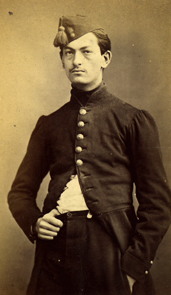
\includegraphics[width=\linewidth]{images/book3/b1-michel-levy.jpg}

{\scriptsize Michel-Lévy sebagai mahasiswa, sekitar 1862. Domain publik.}
\end{minipage}
\end{history}

Dua gelombang yang keluar dari suatu butir dapat diberi \omterm{def:b1:optical-mineralogy:retardation}{retardasi} tambahan yang diketahui oleh keping pelengkap yang diletakkan di atas sayatan pada \ang{45} terhadap polarisator. Yang paling umum dipotong untuk memperlihatkan merah \omterm{def:b1:optical-mineralogy:interference-colour}{orde} pertama, \omterm{def:b1:optical-mineralogy:retardation}{retardasi} sekitar \qty{540}{nm}. Bila arah getar lambat butir sejajar arah lambat keping, tundanya bertambah dan warna butir naik sekitar satu \omterm{def:b1:optical-mineralogy:interference-colour}{orde}; bila sejajar arah cepat, keduanya saling mengurangi dan warnanya turun. Butir kelabu \omterm{def:b1:optical-mineralogy:interference-colour}{orde} pertama sebesar \qty{100}{nm} menjadi biru \omterm{def:b1:optical-mineralogy:interference-colour}{orde} kedua (\qty{640}{nm}) pada satu orientasi dan jingga \omterm{def:b1:optical-mineralogy:interference-colour}{orde} pertama (\qty{440}{nm}) pada orientasi lain; uji ini menunjukkan arah getar mana dari dua arah getar butir yang lambat, sifat yang dipakai untuk mengidentifikasi \omterm{def:b1:rock-forming-minerals:mineral}{mineral} berbentuk memanjang.

\section{Mengidentifikasi mineral dalam sayatan tipis}

\begin{definition}[Kembaran, kembaran polisintetik]\label{def:b1:optical-mineralogy:twin}
Sebuah \emph{kembaran}\index{kembaran (kristal)} adalah pertumbuhan bersama dari dua kristal atau lebih dari \omterm{def:b1:rock-forming-minerals:mineral}{mineral} yang sama yang kisinya berhubungan oleh simetri yang tidak dimiliki kristal itu sendiri, seperti pencerminan melalui suatu bidang (bidang kembaran). \emph{Kembaran polisintetik}\index{kembaran polisintetik} adalah kembaran berulang pada bidang-bidang sejajar, yang membagi kristal menjadi lamel-lamel sejajar yang tipis dengan orientasi bergantian.
\end{definition}

Di antara polarisator silang lamel-lamel \omterm{def:b1:optical-mineralogy:twin}{kembaran polisintetik} padam bergantian: separuhnya gelap ketika separuh lainnya terang, dan kristal tampak bergaris. \omterm{def:b1:rock-forming-minerals:groups}{Plagioklas} hampir selalu memperlihatkan garis-garis ini, yang membedakannya seketika dari kuarsa dan \omterm{def:b1:rock-forming-minerals:groups}{feldspar alkali}; ciri lainnya, relief rendah dan warna kelabu hingga putih \omterm{def:b1:optical-mineralogy:interference-colour}{orde} pertama, ia miliki bersama mereka. \omterm{def:b1:optical-mineralogy:extinction}{Sudut pemadaman} kedua himpunan lamel, diukur di kedua sisi bidang \omterm{def:b1:optical-mineralogy:twin}{kembaran}, bergantung pada komposisi \omterm{def:b1:rock-forming-minerals:groups}{plagioklas}, dan bagan sudut itu memberikan kandungan anortitnya.

\begin{method}[Mengidentifikasi mineral dalam sayatan tipis]\label{met:b1:optical-mineralogy:identify}
\begin{enumerate}
  \item Dalam \omterm{def:b1:field-lab-methods-1:microscope}{cahaya terpolarisasi bidang}: catat apakah butir itu opak; warna dan \omterm{def:b1:optical-mineralogy:pleochroism}{pleokroismenya} (putar meja); reliefnya, dan di sisi mana dari $1.54$ indeksnya berada (\omterm{def:b1:optical-mineralogy:relief}{garis Becke}); bentuk dan belahannya, serta sudut antara dua belahan.
  \item Di antara polarisator silang: periksa apakah ia tetap gelap (isotropik, atau penampang tegak lurus \omterm{def:b1:optical-mineralogy:optic-axis}{sumbu optik}); di antara butir \omterm{def:b1:rock-forming-minerals:mineral}{mineral} yang sama, carilah \omterm{def:b1:optical-mineralogy:interference-colour}{warna interferensi} tertinggi dan bacalah \omterm{def:b1:optical-mineralogy:birefringence}{birefringensi} pada \omterm{def:b1:optical-mineralogy:interference-colour}{diagram Michel-Lévy} untuk tebal sayatan.
  \item Ukur \omterm{def:b1:optical-mineralogy:extinction}{sudut pemadaman} pada butir yang memperlihatkan belahan atau pemanjangan; carilah \omterm{def:b1:optical-mineralogy:twin}{kembaran} (garis polisintetik, \omterm{def:b1:optical-mineralogy:twin}{kembaran} sederhana).
  \item Bandingkan dengan tabel sifat optik (\cref{tab:b1:optical-mineralogy:key}) dan dengan \omterm{def:b1:rock-forming-minerals:mineral}{mineral} yang dapat dikandung batuan (\cref{ch:b1:rock-forming-minerals}).
\end{enumerate}
\end{method}

\begin{table}[htbp]
\centering\footnotesize
\setlength{\tabcolsep}{3pt}
% ledger: hom:quartz-optics, hom:orthoclase-optics, hom:albite-optics, hom:anorthite-optics, hom:muscovite-optics, hom:biotite-optics, hom:hornblende-optics, hom:diopside-optics, hom:forsterite-optics, hom:fayalite-optics, hom:almandine-optics, hom:calcite-optics, hom:magnetite-optics
\begin{tabular}{@{}>{\raggedright\arraybackslash}p{2.0cm}>{\raggedright\arraybackslash}p{2.6cm}>{\raggedright\arraybackslash}p{2.3cm}>{\raggedright\arraybackslash}p{1.8cm}>{\raggedright\arraybackslash}p{3.0cm}>{\raggedright\arraybackslash}p{3.8cm}@{}}
\hline
\omterm{def:b1:rock-forming-minerals:mineral}{mineral} & warna (PPL) & indeks & \omterm{def:b1:optical-mineralogy:birefringence}{birefringensi} & warna tertinggi pada \qty{30}{\micro m} & ciri lain \\
\hline
kuarsa & tak berwarna & 1.544--1.553 & 0.009 & putih \omterm{def:b1:optical-mineralogy:interference-colour}{orde} pertama & tanpa belahan; tanpa \omterm{def:b1:optical-mineralogy:twin}{kembaran} terlihat; \omterm{def:b1:optical-mineralogy:optic-axis}{uniaksial} \\
ortoklas & tak berwarna, sering keruh & 1.518--1.525 & 0.005 & kelabu \omterm{def:b1:optical-mineralogy:interference-colour}{orde} pertama & relief negatif; \omterm{def:b1:optical-mineralogy:twin}{kembaran} sederhana \\
\omterm{def:b1:rock-forming-minerals:groups}{plagioklas} & tak berwarna & 1.526--1.590 & 0.008--0.013 & putih hingga kuning pucat \omterm{def:b1:optical-mineralogy:interference-colour}{orde} pertama & \omterm{def:b1:optical-mineralogy:twin}{kembaran polisintetik} \\
muskovit & tak berwarna & 1.552--1.618 & 0.035--0.042 & \omterm{def:b1:optical-mineralogy:interference-colour}{orde} kedua hingga ketiga yang cerah & satu belahan sempurna; pemadaman lurus \\
biotit & cokelat, hijau & 1.565--1.696 & 0.04--0.07 & tertutup oleh warnanya sendiri & \omterm{def:b1:optical-mineralogy:pleochroism}{pleokroisme} kuat; satu belahan sempurna \\
hornblende & hijau, cokelat & 1.675--1.695 & 0.020 & biru \omterm{def:b1:optical-mineralogy:interference-colour}{orde} kedua & \omterm{def:b1:optical-mineralogy:pleochroism}{pleokroik}; belahan pada \ang{56}/\ang{124}; pemadaman \ang{15}--\ang{19} \\
diopsid & tak berwarna & 1.664--1.694 & 0.030 & kuning \omterm{def:b1:optical-mineralogy:interference-colour}{orde} kedua & belahan pada sekitar \ang{87}/\ang{93}; pemadaman sekitar \ang{38} \\
\omterm{def:b1:rock-forming-minerals:groups}{olivin} & tak berwarna (Mg) hingga kuning pucat (Fe) & 1.635--1.879 & 0.035--0.052 & ujung \omterm{def:b1:optical-mineralogy:interference-colour}{orde} kedua hingga \omterm{def:b1:optical-mineralogy:interference-colour}{orde} ketiga & relief tinggi; retakan tak beraturan, tanpa belahan baik \\
\omterm{def:b1:rock-forming-minerals:groups}{garnet} & tak berwarna hingga merah muda pucat & 1.830 (almandin) & isotropik & hitam & relief sangat tinggi; garis tepi enam atau delapan sisi \\
kalsit & tak berwarna & 1.486--1.658 & 0.172 & putih \omterm{def:b1:optical-mineralogy:interference-colour}{orde} tinggi & relief berubah ketika diputar; belahan rombohedral \\
magnetit & opak & --- & --- & --- & hitam dalam kedua cahaya \\
\hline
\end{tabular}
\caption{Sifat optik \omterm{def:b1:rock-forming-minerals:mineral}{mineral} pembentuk batuan yang umum dalam \omterm{def:b1:field-lab-methods-1:thin-section}{sayatan tipis}.
PPL: \omterm{def:b1:field-lab-methods-1:microscope}{cahaya terpolarisasi bidang}. Warna tertinggi dibaca pada \omterm{def:b1:optical-mineralogy:interference-colour}{diagram Michel-Lévy} pada $\Delta = \qty{30000}{nm}\times\delta$.}
\label{tab:b1:optical-mineralogy:key}
\end{table}

\begin{omfigure}
\setlength{\tabcolsep}{2pt}
\begin{tabular}{cc}
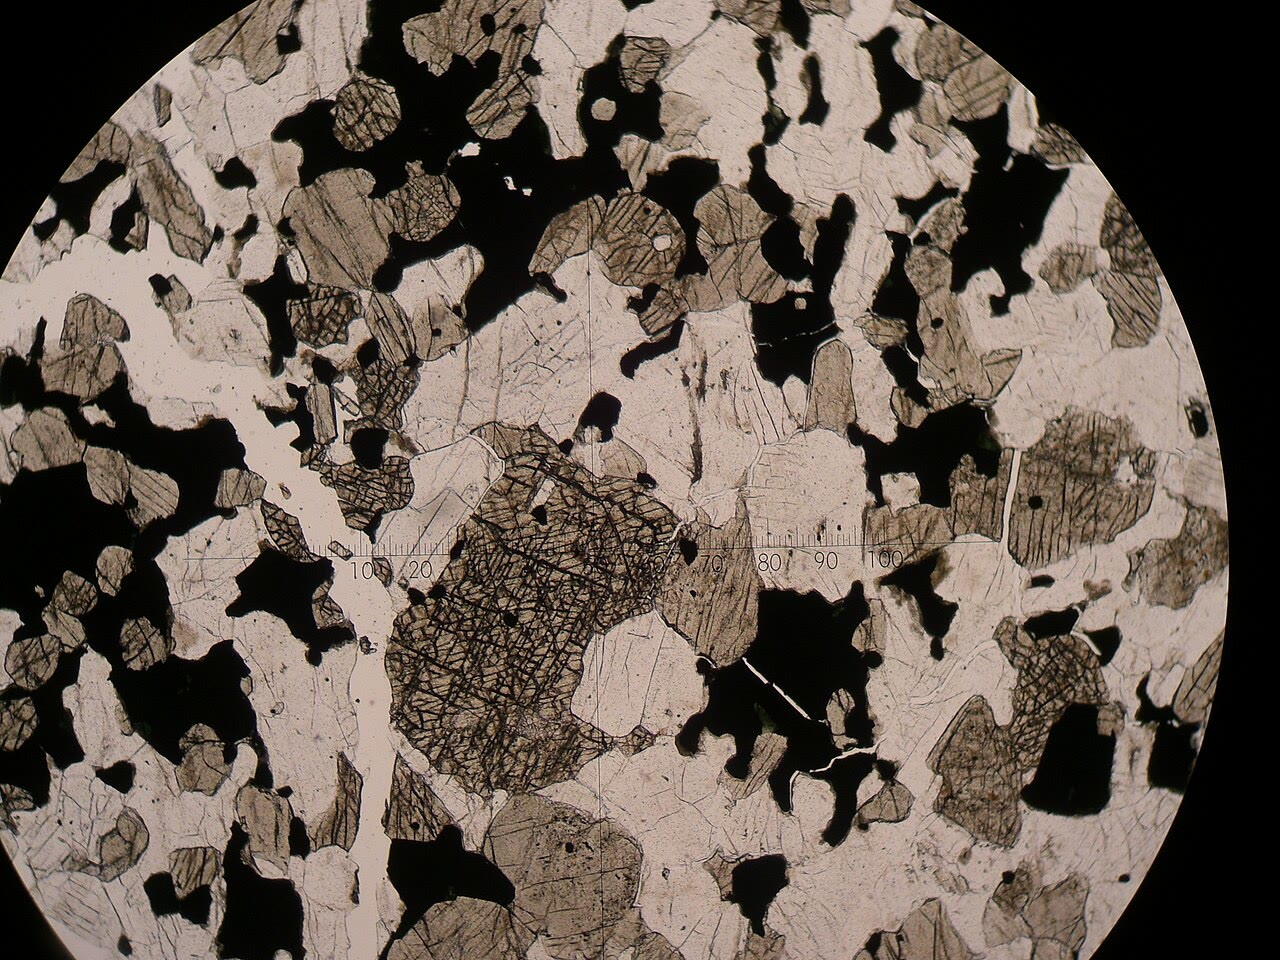
\includegraphics[width=0.485\linewidth]{images/book3/b1-gabbro-ppl.jpg} &
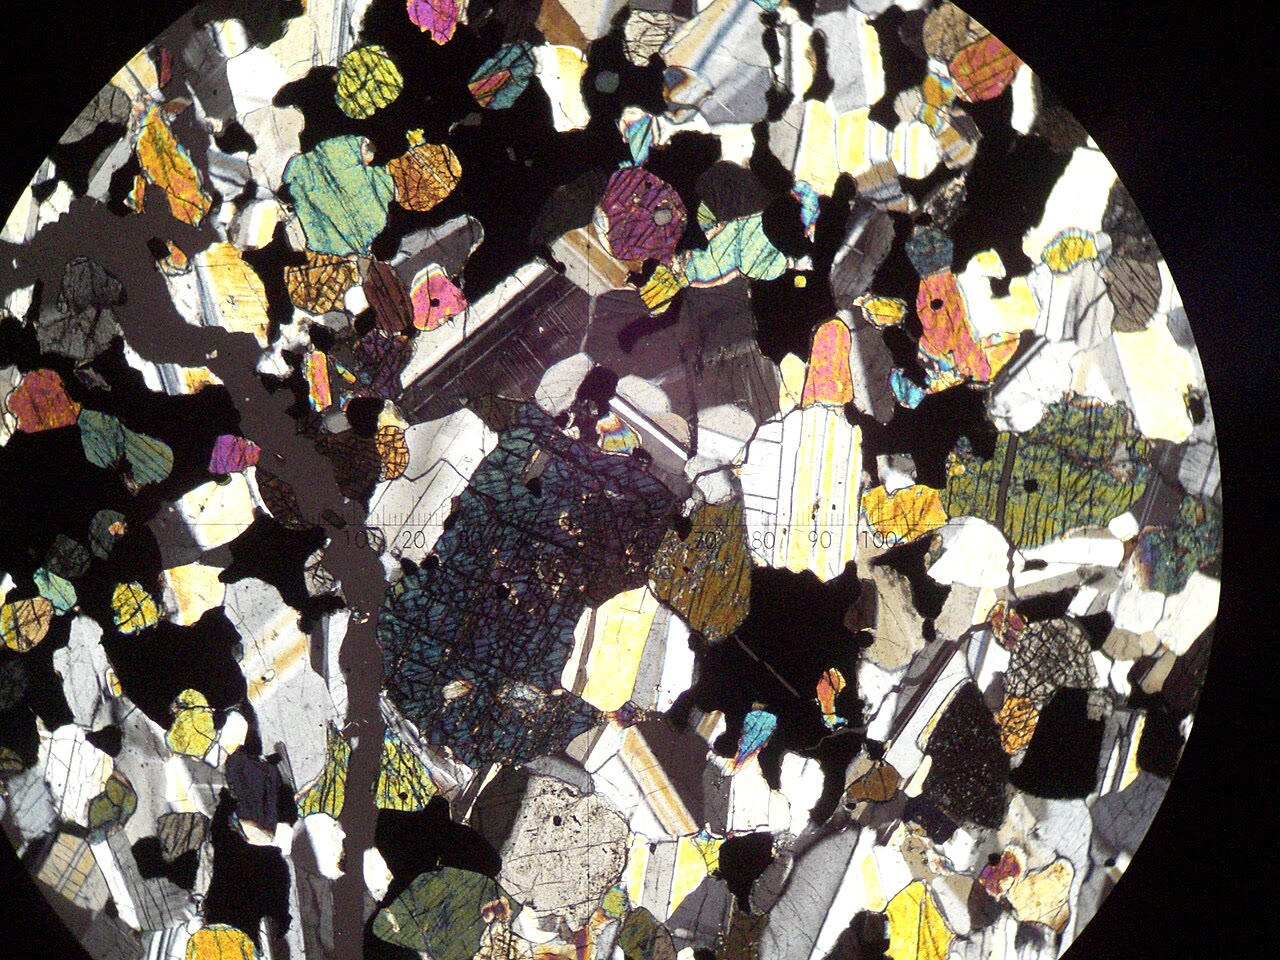
\includegraphics[width=0.485\linewidth]{images/book3/b1-gabbro-xpl.jpg} \\
{\small (a) \omterm{def:b1:field-lab-methods-1:microscope}{cahaya terpolarisasi bidang}} & {\small (b) polarisator silang} \\
\end{tabular}
% ledger: commons:gabbro-ppl, commons:gabbro-xpl

\medskip
{\small Bidang yang sama dari gabro dalam \omterm{def:b1:field-lab-methods-1:thin-section}{sayatan tipis}. Dalam \omterm{def:b1:field-lab-methods-1:microscope}{cahaya terpolarisasi bidang} (a), \omterm{def:b1:rock-forming-minerals:groups}{plagioklas} tak berwarna dengan relief rendah, butir \omterm{def:b1:rock-forming-minerals:groups}{piroksen} dan \omterm{def:b1:rock-forming-minerals:groups}{olivin} kelabu cokelat pucat dengan relief tinggi dan retakan rapat, dan bijih opak berwarna hitam; skalanya satu mikrometer pada okuler. Di antara polarisator silang (b), lamel \omterm{def:b1:rock-forming-minerals:groups}{plagioklas} bergaris oleh \omterm{def:b1:optical-mineralogy:twin}{kembaran polisintetik}, butir \omterm{def:b1:rock-forming-minerals:groups}{piroksen} dan \omterm{def:b1:rock-forming-minerals:groups}{olivin} bersinar dalam warna \omterm{def:b1:optical-mineralogy:interference-colour}{orde} kedua, dan bijih tetap hitam. Foto Chmee2, CC BY-SA 3.0 (Wikimedia Commons).}
\end{omfigure}

\begin{inthelab}[Sesi di mikroskop]
\begin{minipage}[t]{0.55\linewidth}\vspace{0pt}
Seorang petrolog yang mendeskripsikan \omterm{def:b1:field-lab-methods-1:thin-section}{sayatan tipis} baru mengerjakannya pertama dengan pembesaran rendah, untuk melihat tekstur dan \omterm{def:b1:rock-forming-minerals:mineral}{mineral} utama, lalu butir demi butir. Untuk setiap \omterm{def:b1:rock-forming-minerals:mineral}{mineral} ia mencatat pengamatan dengan metode di atas, memperkirakan proporsinya di lapangan, dan mencatat bagaimana butir-butirnya bersentuhan: mana yang mengkristal lebih dulu, mana yang mengisi ruang yang tersisa, mana yang menggantikan yang lain. Pengukuran cahaya dilakukan dengan meja berskala derajat dan keping pelengkap; komposisi, bila penting, diukur kemudian dengan mikroprobe pada sayatan yang sama. Laboratorium pengajaran bekerja dengan cara yang sama, satu mikroskop per mahasiswa dan sekotak sayatan acuan \omterm{def:b1:rock-forming-minerals:mineral}{mineral} yang diketahui di sampingnya.
\end{minipage}\hfill
\begin{minipage}[t]{0.42\linewidth}\vspace{0pt}
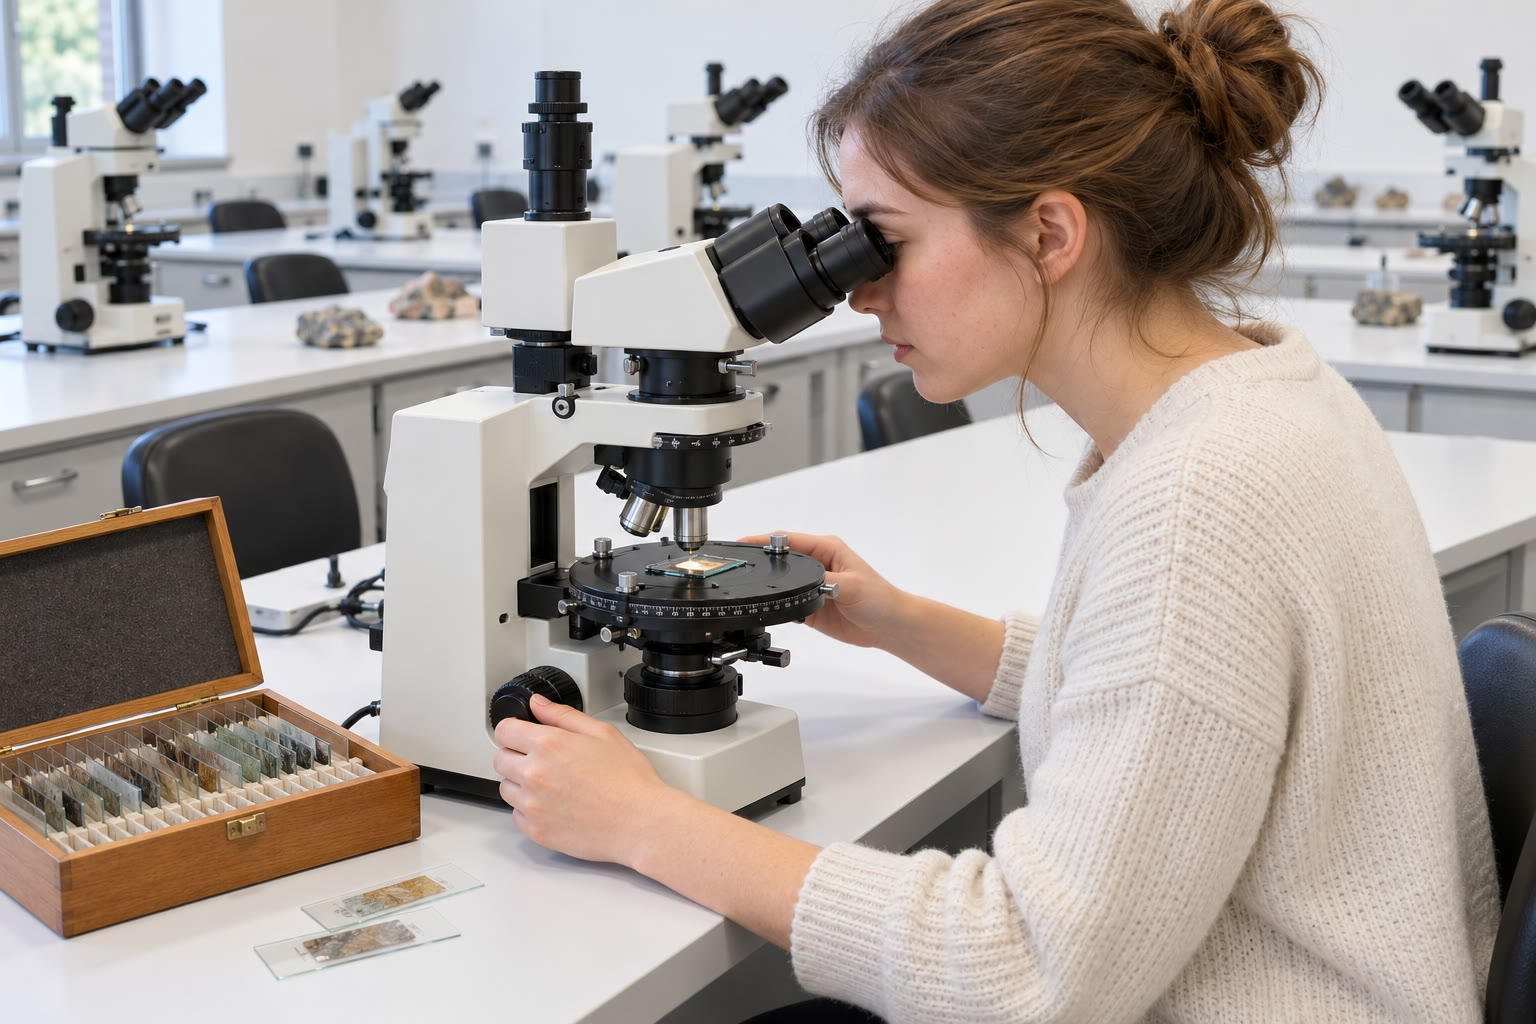
\includegraphics[width=\linewidth]{images/book3/ai/b1-microscope-student.jpg}

{\scriptsize Seorang mahasiswa di \omterm{def:b1:field-lab-methods-1:microscope}{mikroskop polarisasi} di laboratorium pengajaran (ilustrasi buatan AI).}
\end{minipage}
\end{inthelab}

\section{Latihan}

\begin{exercise}[$\star$]\label{exo:b1:optical-mineralogy:1}
Hitunglah \omterm{def:b1:optical-mineralogy:retardation}{retardasi} terbesar kuarsa ($\delta = 0.009$) dan kalsit ($\delta = 0.172$) dalam sayatan setebal \qty{30}{\micro m}. Dengan \omterm{def:b1:optical-mineralogy:interference-colour}{diagram Michel-Lévy}, gambarkan warna masing-masing.
% ledger: hom:quartz-optics, hom:calcite-optics
\end{exercise}

\begin{exercise}[$\star$]\label{exo:b1:optical-mineralogy:2}
Sebuah butir diputar pada meja di antara polarisator silang. Hitunglah $I/I_0$, sebagai pecahan dari maksimumnya, pada $\theta = 0$, \ang{22.5}, \ang{45}, \ang{67.5} dan \ang{90} dari \omterm{def:b1:optical-mineralogy:extinction}{posisi pemadaman}.
\end{exercise}

\begin{exercise}[$\star$]\label{exo:b1:optical-mineralogy:3}
Jelaskan mengapa \omterm{def:b1:rock-forming-minerals:groups}{garnet} tetap hitam di antara polarisator silang apa pun posisi mejanya, dan mengapa butir kuarsa mungkin melakukan hal yang sama. Bagaimana kedua \omterm{def:b1:rock-forming-minerals:mineral}{mineral} itu dibedakan dalam \omterm{def:b1:field-lab-methods-1:microscope}{cahaya terpolarisasi bidang}?
\end{exercise}

\begin{exercise}[$\star$]\label{exo:b1:optical-mineralogy:4}
Urutkan menurut relief, dalam pemasang berindeks $1.54$, ortoklas ($n$ sekitar $1.52$), kuarsa ($1.55$), forsterit ($1.65$), dan almandin ($1.83$). Yang mana memiliki relief negatif? Ke arah mana \omterm{def:b1:optical-mineralogy:relief}{garis Becke-nya} bergerak ketika fokus dinaikkan?
% ledger: hom:orthoclase-optics, hom:quartz-optics, hom:forsterite-optics, hom:almandine-optics
\end{exercise}

\begin{exercise}[$\star\star$]\label{exo:b1:optical-mineralogy:5}
Pada sayatan \qty{30}{\micro m}, butir-butir \omterm{def:b1:rock-forming-minerals:mineral}{mineral} hijau \omterm{def:b1:optical-mineralogy:pleochroism}{pleokroik} dengan dua belahan pada \ang{56} dan \ang{124} hanya menunjukkan biru \omterm{def:b1:optical-mineralogy:interference-colour}{orde} kedua paling tinggi, dibaca pada bagan sebagai $\Delta = \qty{650}{nm}$. Hitunglah \omterm{def:b1:optical-mineralogy:birefringence}{birefringensinya} dan namai \omterm{def:b1:rock-forming-minerals:mineral}{mineral} itu dengan \cref{tab:b1:optical-mineralogy:key}.
\end{exercise}

\begin{exercise}[$\star\star$]\label{exo:b1:optical-mineralogy:6}
Dengan memakai \cref{prop:b1:optical-mineralogy:relief} dengan $n_m = 1.54$ dan $i = \ang{30}$, hitunglah deviasi di tepi butir kuarsa ($n = 1.553$) dan butir forsterit ($n = 1.651$), dalam derajat, dan perbandingan keduanya. Periksa yang kedua dengan hukum Snell secara tepat.
\end{exercise}

\begin{exercise}[$\star\star$]\label{exo:b1:optical-mineralogy:7}
Sebuah keping merah \omterm{def:b1:optical-mineralogy:interference-colour}{orde} pertama memiliki $\Delta = \qty{540}{nm}$. Sebuah butir kuarsa dengan $\Delta = \qty{270}{nm}$ diletakkan pada \ang{45} dengan keping dimasukkan. Berapakah kedua \omterm{def:b1:optical-mineralogy:retardation}{retardasi} total yang mungkin, dan warna yang diberikannya pada bagan? Orientasi mana yang membuat kedua arah lambat sejajar?
\end{exercise}

\begin{exercise}[$\star\star$]\label{exo:b1:optical-mineralogy:8}
Pada tepinya yang meruncing, sebuah butir fayalit ($\delta = 0.052$) menipis dari \qty{30}{\micro m} hingga nol. Berapa rona merah-ungu, yang mengakhiri \omterm{def:b1:optical-mineralogy:interference-colour}{orde} pada 542, 1074 dan \qty{1605}{nm}, muncul sebagai pita berwarna di antara tepi dan bagian tebal penuh butir?
% ledger: hom:fayalite-optics
\end{exercise}

\begin{exercise}[$\star\star$]\label{exo:b1:optical-mineralogy:9}
Pada beberapa butir memanjang dengan satu belahan baik, seorang ahli geologi mengukur \omterm{def:b1:optical-mineralogy:extinction}{sudut pemadaman} \ang{0}, \ang{21}, \ang{36} dan \ang{37} antara jejak belahan dan arah getar lambat. Mengapa nilainya berbeda? Apakah \omterm{def:b1:rock-forming-minerals:mineral}{mineral} itu lebih mungkin diopsid atau hornblende?
% ledger: hom:diopside-optics, hom:hornblende-optics
\end{exercise}

\begin{exercise}[$\star\star\star$]\label{exo:b1:optical-mineralogy:10}
Ulangi pembuktian \cref{thm:b1:optical-mineralogy:intensity} dengan analisator sejajar polarisator, dan tunjukkan bahwa $I_\parallel = I_0\bigl(1 - \sin^2 2\theta\sin^2(\pi\Delta/\lambda)\bigr)$. Warna apa yang ditunjukkan butir $\Delta = \qty{550}{nm}$ pada \ang{45} di antara polarisator sejajar?
\end{exercise}

\begin{exercise}[$\star\star\star$]\label{exo:b1:optical-mineralogy:11}
Untuk sebuah butir kalsit dengan $\Delta = \qty{5000}{nm}$, faktor $\sin^2(\pi\Delta/\lambda)$ menghilang setiap kali $\Delta/\lambda$ adalah bilangan bulat. (a) Berapa kali ia menghilang antara \num{400} dan \qty{700}{nm}? (b) Tunjukkan bahwa di dekat $\lambda = \qty{550}{nm}$ dua nol berturut-turut berjarak sekitar $\lambda^2/\Delta$, dan hitunglah. (c) Jelaskan mengapa butir itu tampak hampir putih.
\end{exercise}

\begin{exercise}[$\star\star\star$]\label{exo:b1:optical-mineralogy:12}
Tunjukkan bahwa, dirata-ratakan atas satu putaran penuh meja, butir di antara polarisator silang meneruskan $\frac12 I_0\sin^2(\pi\Delta/\lambda)$. Seorang ahli geologi memperkirakan \omterm{def:b1:optical-mineralogy:birefringence}{birefringensi} dari warna tertinggi setiap \omterm{def:b1:rock-forming-minerals:mineral}{mineral}, dengan menganggap \qty{30}{\micro m}, pada sayatan yang sebenarnya setebal \qty{25}{\micro m}. Dengan faktor berapakah semua nilainya keliru, dan ke arah mana?
\end{exercise}

\section{Soal: Mengidentifikasi mineral sayatan tipis tak dikenal}

\begin{problem}[{Soal akhir pekan --- mengamati relief, pleokroisme dan warna interferensi, mengukur tebal sayatan dengan kuarsa, dan menamai mineralnya}]
\label{pb:b1:optical-mineralogy:1}
% nilai: calc/ch08.py; data optik: ledger hom:*-optics
% ledger: hom:quartz-optics, hom:diopside-optics, hom:forsterite-optics, hom:albite-optics, hom:anorthite-optics, hom:hornblende-optics, hom:biotite-optics
Sebuah \omterm{def:b1:field-lab-methods-1:thin-section}{sayatan tipis} batuan beku tak dikenal, dipasang dalam resin berindeks $1.540$, dikatakan setebal \qty{30}{\micro m}. Ia mengandung lima \omterm{def:b1:rock-forming-minerals:mineral}{mineral}, diberi label A sampai E. Gunakan tabel sifat optik bab ini, \omterm{def:b1:optical-mineralogy:interference-colour}{diagram Michel-Lévy}, dan nilai-nilai berikut: kuarsa $n_\omega = 1.544$, $n_\varepsilon = 1.553$; diopsid $n_\alpha = 1.664$, $n_\beta = 1.672$, $n_\gamma = 1.694$.

\medskip
\noindent\textbf{Bagian I --- Cahaya terpolarisasi bidang.}
\begin{enumerate}
  \item \omterm{def:b1:rock-forming-minerals:mineral}{Mineral} A tak berwarna, dengan batas butir sulit dilihat. \omterm{def:b1:rock-forming-minerals:mineral}{Mineral} B tak berwarna, dengan tepi gelap tebal dan dua belahan yang bertemu pada sekitar \ang{87}. Yang mana memiliki relief lebih tinggi?
  \item Untuk A, dianggap kuarsa, dan B, dianggap diopsid, hitunglah $|n - n_m|$ dengan memakai rata-rata indeks utama masing-masing.
  \item Dengan memakai \cref{prop:b1:optical-mineralogy:relief}, hitunglah perbandingan deviasi di tepi mereka untuk gradien batas yang sama.
  \item Ketika fokus dinaikkan, \omterm{def:b1:optical-mineralogy:relief}{garis Becke} dari B bergerak ke dalam butir. Apa yang ditunjukkan ini?
  \item \omterm{def:b1:rock-forming-minerals:mineral}{Mineral} C berubah dari kuning pucat menjadi cokelat gelap ketika meja berputar, paling gelap ketika belahan tunggalnya sejajar polarisator. Sebutkan sifatnya dan \omterm{def:b1:rock-forming-minerals:mineral}{mineralnya}.
  \item \omterm{def:b1:rock-forming-minerals:mineral}{Mineral} D tak berwarna, dengan relief rendah, dalam bilah panjang; E hijau hingga kuning dan \omterm{def:b1:optical-mineralogy:pleochroism}{pleokroik}, dengan dua belahan pada \ang{124}. Apa yang disarankan sudut itu untuk E?
\end{enumerate}

\medskip
\noindent\textbf{Bagian II --- Tebal sayatan.}
\begin{enumerate}[resume]
  \item Berapakah \omterm{def:b1:optical-mineralogy:retardation}{retardasi} terbesar kuarsa dalam sayatan persis \qty{30}{\micro m}? Warna apa yang ditunjukkannya?
  \item Mengapa \omterm{def:b1:optical-mineralogy:retardation}{retardasi} terbesar harus dicari di antara banyak butir A, bukan diukur pada salah satu dari mereka?
  \item Warna tertinggi yang ditunjukkan butir-butir A adalah kuning pucat \omterm{def:b1:optical-mineralogy:interference-colour}{orde} pertama; komparator baji kuarsa memberikan \omterm{def:b1:optical-mineralogy:retardation}{retardasinya} sebagai \qty{342}{nm}. Hitunglah tebal sebenarnya sayatan.
  \item Dengan berapa persen sayatan itu lebih tebal daripada seharusnya?
  \item Pada $\lambda = \qty{550}{nm}$ dan \ang{45} dari pemadaman, hitunglah $I/I_0$ untuk butir kuarsa ini, dan untuk butir yang sama dalam sayatan setebal \qty{30}{\micro m}.
  \item Hitunglah rentang \omterm{def:b1:optical-mineralogy:retardation}{retardasi} D, dianggap \omterm{def:b1:rock-forming-minerals:groups}{plagioklas} ($\delta = 0.008$ sampai $0.013$), dalam sayatan ini, dan katakan apakah warnanya tetap di \omterm{def:b1:optical-mineralogy:interference-colour}{orde} pertama.
\end{enumerate}

\medskip
\noindent\textbf{Bagian III --- Birefringensi B.}
\begin{enumerate}[resume]
  \item Warna tertinggi B adalah biru yang dibaca sebagai $\Delta = \qty{1140}{nm}$. Dalam \omterm{def:b1:optical-mineralogy:interference-colour}{orde} berapakah ia?
  \item Hitunglah \omterm{def:b1:optical-mineralogy:birefringence}{birefringensi} B dengan tebal yang ditemukan pada soal 9.
  \item \omterm{def:b1:optical-mineralogy:birefringence}{Birefringensi} apa yang akan ditemukan bila dianggap \qty{30}{\micro m}? \omterm{def:b1:rock-forming-minerals:mineral}{Mineral} tak berwarna berelief tinggi mana yang akan disarankannya, dan mengapa ia tidak cocok dalam batuan dengan kuarsa (pertimbangkan \ce{Mg2SiO4 + SiO2 -> 2 MgSiO3})?
  \item Bandingkan hasil soal 14 dengan tabel, bersama dengan relief dan belahan B, dan simpulkan.
  \item Warna apa yang paling tinggi ditunjukkan B dalam sayatan \qty{30}{\micro m} yang benar?
  \item Sayatan itu digerinda hingga \qty{30}{\micro m}. Berapa banyak ia harus ditipiskan, dan berapakah warna tertinggi kuarsa kemudian?
\end{enumerate}

\medskip
\noindent\textbf{Bagian IV --- Pemadaman dan kembaran.}
\begin{enumerate}[resume]
  \item Lath D terbagi menjadi garis-garis sejajar yang padam bergantian. Sebutkan ciri itu dan \omterm{def:b1:rock-forming-minerals:mineral}{mineralnya}.
  \item Garis-garis satu bilah padam pada \ang{27} dan \ang{28} di kedua sisi bidang \omterm{def:b1:optical-mineralogy:twin}{kembaran}. Apa yang diberikan sudut-sudut seperti itu, yang diukur pada banyak bilah, bila dibandingkan dengan bagan yang diterbitkan?
  \item \omterm{def:b1:optical-mineralogy:extinction}{Sudut pemadaman} tertinggi antara belahan E dan arah getar lambatnya adalah \ang{17}. Namai E.
  \item Hitunglah \omterm{def:b1:optical-mineralogy:retardation}{retardasi} terbesar E dalam sayatan ini dan warna yang ditunjukkannya.
  \item Sebuah butir B tetap gelap selama satu putaran penuh. Jelaskan bagaimana ia dapat merupakan \omterm{def:b1:rock-forming-minerals:mineral}{mineral} yang sama dengan butir B yang terang.
  \item Daftarkan \omterm{def:b1:rock-forming-minerals:mineral}{mineral} A sampai E, dan katakan jenis batuan apa yang mereka bentuk.
  \item Berapakah tebal sebenarnya sayatan, dalam mikrometer?
\end{enumerate}
\end{problem}
